\documentclass[dvipsnames]{article}
\usepackage[utf8]{inputenc}
\usepackage[left=3cm, right=3cm, top=2cm]{geometry}
\title{Dynamic Boundary Conditions}
\author{Silvin Willemsen}
\date{June 2020}

\usepackage{natbib}
\usepackage{graphicx}
\usepackage{appendix}
\usepackage{amsmath}
\usepackage{amsfonts}
\usepackage{amssymb}

\usepackage{xcolor}
\def\SBcomment[#1]{\textcolor{red}{#1}}
\def\SWcomment[#1]{\textcolor{blue}{#1}}
\def\SScomment[#1]{\textcolor{green}{#1}}
\def\type[#1]{\textcolor{purple}{#1}}

\begin{document}
\maketitle

\section{Introduction}
This document shows the work done and documentation on dynamic boundary conditions.

\section{Explanation}
Let's take the 1D wave equation in discrete time:
\begin{equation}
    \delta_{tt}u_l^n=c^2\delta_{xx}u_l^n
\end{equation}
with simply supported boundary conditions such that
\begin{equation}
u_l^n = \delta_{xx}u_l^n = 0 \quad \text{at} \quad l = 0, N.
\end{equation}




The question is then, how do we modulate $u_0^n$ so that the boundary condition at $x=0$ is satisfied if $u_0^n$ is not at that location?

Through stability analysis one can arrive at a condition for the grid spacing that needs to be satisfied in order for the implementation to be stable. In this case this is
\begin{equation}\label{eq:stabilityCondition}
    h \geq ck,
\end{equation}
the closer $h$ is to this condition, the more accurate the scheme will be. 
Consider a string with a wavespeed of $c = 1470$ m/s. With $f_\text{s} = 44100$ we can satisfy condition \eqref{eq:stabilityCondition} with equality $h = 0.333$.

\begin{figure}[h]
\centerline{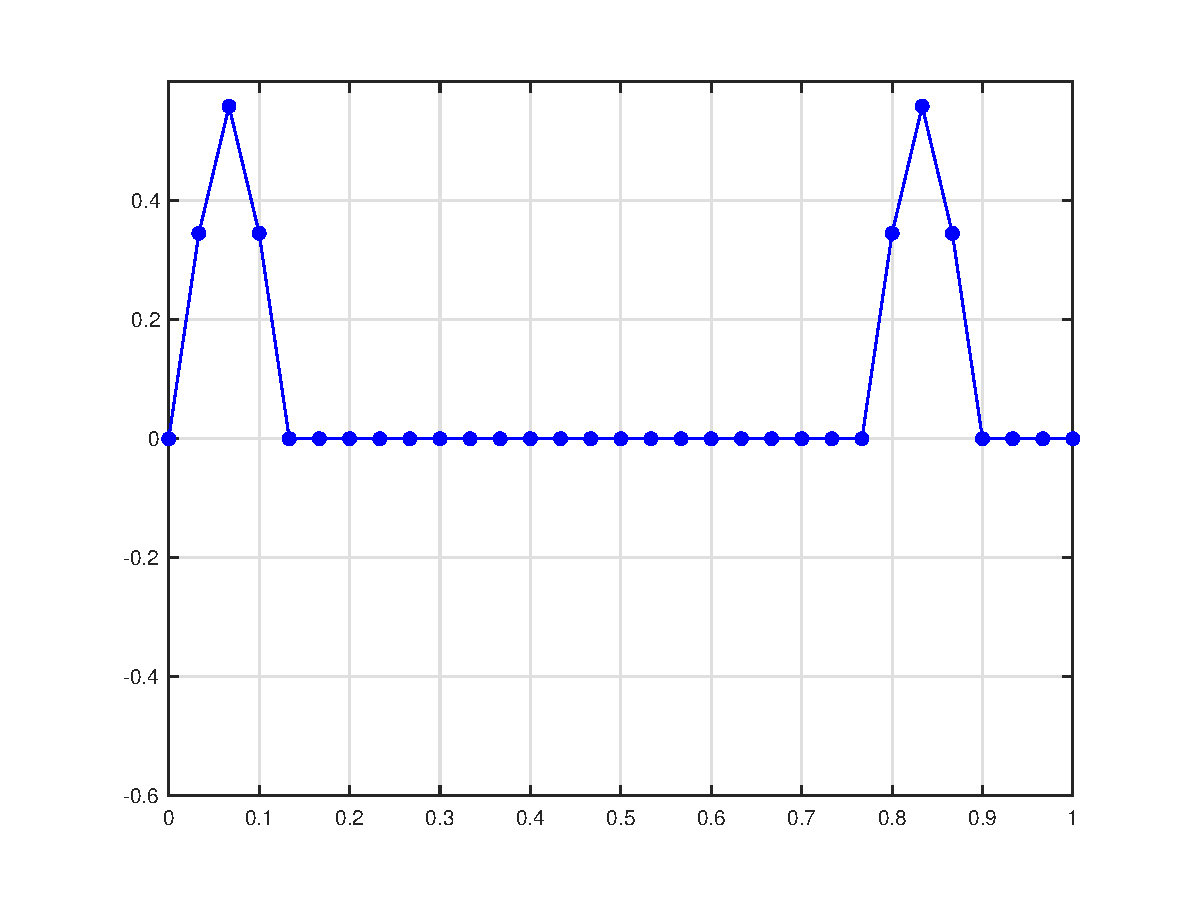
\includegraphics[width=0.6\columnwidth]{plot1.eps}}
\caption{\label{fig:eta}{String $N=30$.}}
\end{figure}

\begin{figure}[h]
\centerline{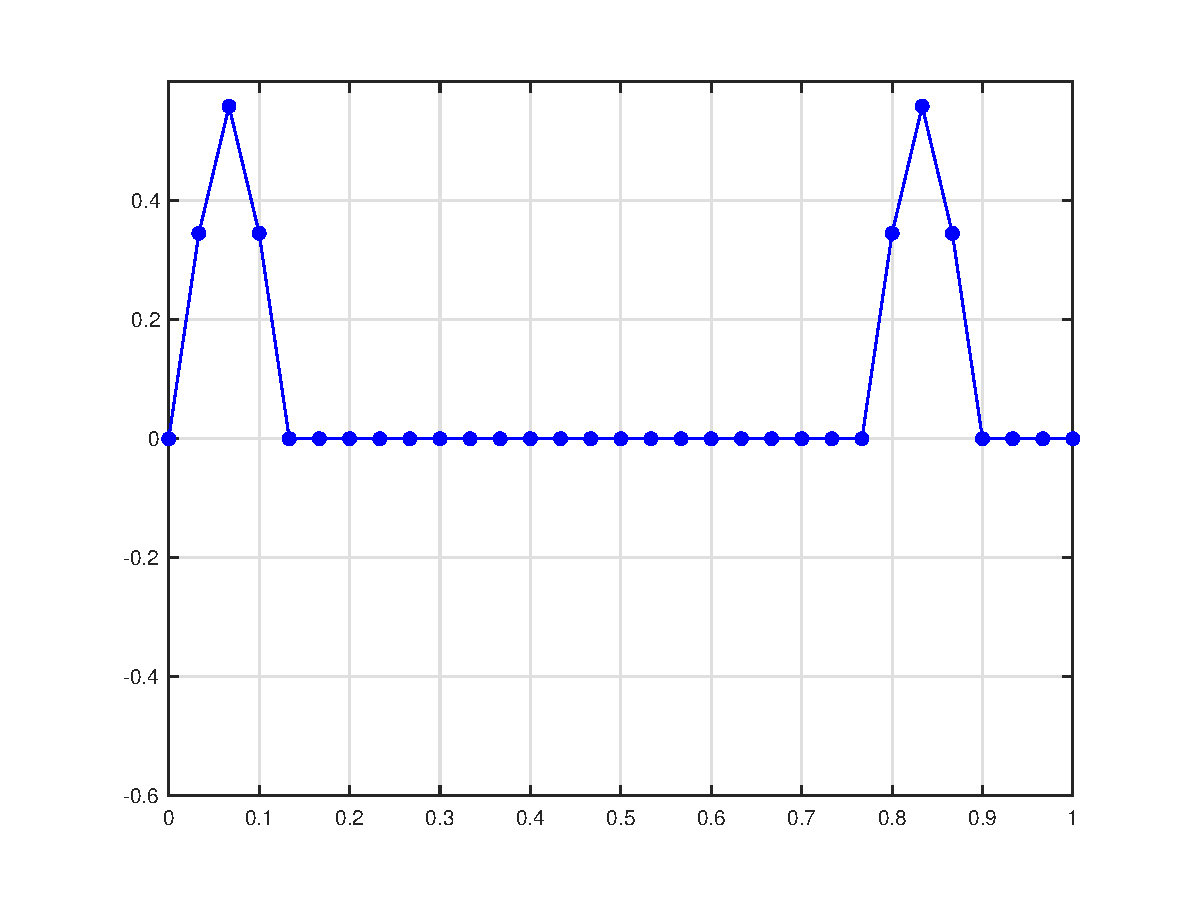
\includegraphics[width=0.6\columnwidth]{plot1.eps}}
\caption{\label{fig:eta}{String $N=30$.}}
\end{figure}

\end{document}
